%===================================== CHAP 4 =================================

\chapter{Technology}
% ========================== section ============================
\section{Framework - Theano}

Theano is a Python library for building high-performance mathematical tools. It lets you write library-specific code which will then be analyzed, optimized, and compiled to C and optionally CUDA, the latter enabling execution of code on a GPU which supports CUDA. Because of the decentralized nature of ANNs, training and executing ANNs on GPUs may drastically improve performance, and Theano lets you symbolically define the algorithms in a high-level programming environment. In this thesis I will use Theano to implement the ANN model and experiments that is outlined in chapter \ref{future_work}. For those familiar with Mathematica, symbolic definitions using Theano are very similar.

\subsection{A Brief Overview}

Theano is tightly integrated with NumPy, another Python package for scientific computation. Moreover, Theano supports parsing several NumPy objects to objects which Theano will be able to use in its optimization process. Which brings us to the compilation process.
Theano operates on symbolic constructs, called tensors; general mathematical constructs. So in order to define a function, you would write the actual mathematical expression, for instance:

\begin{verbatim}
import theano.tensor as T
import theano

A = T.fmatrix('A')
x = T.fvector('x')
b = T.fvector('b')
y = Ax + b

f = theano.function([A, x, b], y)
\end{verbatim}

Before calling the library's function theano.function, which analyses the symbolic expression and constructs executable code from it. To further demonstrate the flexibility of using symbolic expressions, an example of calculating numbers of the Fibonacci sequence is included below (the imports as above being presumed):

\begin{verbatim}
def fib_acc(old, older):
    return old + older

fib_expr, updates = theano.scan(
    fib_acc,
    sequences=None,
    outputs_info=[dict(initial=np.int32([0, 1]), 
    taps=[-1, -2])], n_steps=n)

f_fib_scan = theano.function([n], fib_expr)
\end{verbatim}

Note that the recursive definition is captured by theano.function. When theano.function is called, the first parameter it takes is the input parameters for the function that is to be calculated. 
Preceeding the input parameters are the output parameters, which are the expressions to be calculated. One may also specify among others expressions \textit{updates} for new shared variables that are to be updated by providing 'updates' = [variables] to the function, and \textit{givens} for substitutions that may be made in the computation graph (i.e. if a function should be substituted with a given value instead).
Furthermore, in order to loop over a function, the \textit{scan}-function of the Theano-library may be used. Scan performs an optimized looping over a symbolic graph, letting the user define parameters for optimizing the iteration. For instance it lets the user tell Theano that some variables do not need to be stored, thus re-using a register for the variable as it is updated, potentially speeding up the loop.
Note that Theano may take a normal Python function-object as an input function to the scan-operator. Standard Python code of the f\_fib\_scan loop would be to call fib\_acc(...) in a for-loop. Furthermore, scan lets explicitly define recursive relationships for output expressions that are to be calculated using the taps-variable, which here states that the two former variables are to be kept in memory. Note that this requires one to define the initial values of the parameters.

When defining symbolic expressions such as functions using Theano, Theano constructs a graph of the provided symbolic expressions, see figure \ref{fig:theano_graph_demo}. This allows for differentiation and manipulation through a syntactic and semantic analysis of the resulting graph, optimizing the graph for expression evaluation and graph traversal for code generation. Furthermore, the compiler may then generate optimized code, compiling it according to the provided environmental parameters. This leads to highly efficient C or CUDA executable code.
Note, however, that as the library provides a high-level abstraction for generation of efficient C or CUDA-code, this renders debugging somewhat harder. More specifically, the executable code will be further processed from that in Python and Theano. This means that the programmer may need to predict more about how the code will be compiled, making it highly recommendable or necessary to have some previous knowledge within C and/or how the Python-library's compilation process works.

\begin{figure}
\centering
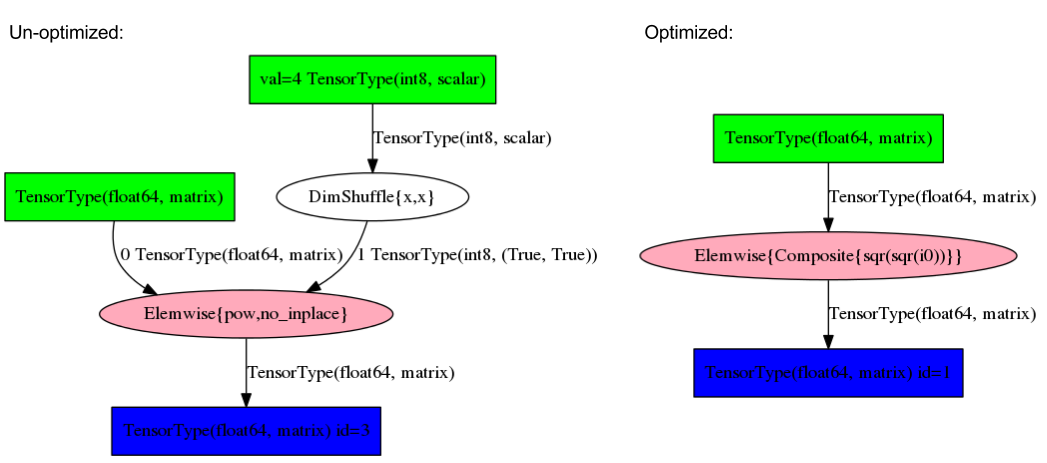
\includegraphics[width=10cm]{fig/unopt_opt_theano_graph}
\caption{Graph manipulation of tensors in Theano during the optimization and compilation process of the expression $y = x^2$.}
\label{fig:theano_graph_demo}
\end{figure}

\subsection{Setup}

In order to use Theano, certain dependencies need to be setup. These are fairly straightforward when it comes to compiling to C-code for CPU-execution. However, when compiling the Theano/Python code to CUDA in order to execute it on a GPU, the process becomes less straightforward. In order to compile and run CUDA-code, certain libraries need to be installed, such as for compiling to CUDA. Furthermore, system dependencies need to be setup, and drivers installed for the GPU. In this thesis and preliminary study, I have setup Theano for use with a GPU on a system with an NVIDIA card, using Ubuntu 14.04 LTS. Furthermore, I used the guide found on \\http://deeplearning.net/software/theano/install.html\#install to obtain installation instructions for doing so.

% ========================== section ============================
\section{GPU Optimization}

\subsection{The Parallelism of ANNs}

Theoretically, a fairly complete decentralization of an ANN is viable during the training phase, rendering the algorithm completely parallelizable. This may in practice be achieved using a smart implementation using FFBP, at the cost of a somewhat slower convergence in terms of iterations (however the parallelism does more than outweigh this increase). Decentralization becomes slightly more complex when introducing dual-networks, due to certain criteria for synchronicity. This may result in a need to pass control back to the interpreter, i.e. when non-Theano-library code has to run. Therefore, it is our aim to provide an implementation where neurons may be trained asynchronously or at least with a layer-wise asynchronicity. This will improve the execution time of the experimental model, and reduce the overall time on performing experiments.

\subsection{A Hardware Example}
A modern chip of these days may contain a thousand CUDA cores, each running at over a thousand MHz. As an example, we have compared one of the cheap high-end GPUs such as NVIDIAs GeForce GTX 960 with an i7 CPU running at about 3.2 GHz in a simplified manner.
\\
The GTX 960 has 1024 CUDA cores, each running at a frequency of 1127 MHz (base).

For the trivial case where the algorithm is entirely decentralized, we have that it could perform,

\begin{center}
\begin{math}
    1024 * 1127 = 1 154 048 * 10^6 \text{ operations per second},
\end{math}
\end{center}
whereas the CPU performs about $3.2 * 10^9$ operations per second.
Theoretically making the GPU $\frac{1154048*10^6}{3.2*10^9} = 360.640$ times more efficient.
\\
Now, the crucial point here to note is that using the GPU requires a substantial amount of overhead in order to transfer instructions and data to on-chip memory. Furthermore, the results need to be transferred back into RAM. It is also important to note that if control has to be passed back to the interpreter during run-time execution of a program in Python/Theano, information on the GPU has to be transferred back to memory, before the CPU may continue to perform the required operations, optionally returning 'control' back to the GPU again. This makes the BUS size a possible bottleneck for run-time efficiency, and does in either way introduce a significant time delay for data-bus-transfer during run-time.

Nevertheless, in the best-case scenario, it is only the setup of the algorithm on the GPU and returning the results which will cause bus-traffic. Rendering the few seconds such overhead takes negligible for algorithms which may spend hours executing solely on the CPU. In such a scenario, we may in theory spend an hour doing crunching an algorithm on the CPU, whilst the GPU may execute it in only about ten seconds. This is without the few seconds spent on overhead before and after execution. Note that a few seconds also have to be added in to such an estimation for every time the interpreter needs control over the program. We will not go in depth into such calculations here, as the complexity of the temporal dependencies in the hardware is outside the scope of this thesis. However, we hope that the former simplified example may provide the reader with a gist of the potential performance boost that may be gained by using GPUs and Theano for training ANNs.

Concluding, parallelizing algorithms for running on GPUs may with average modern high-end GPUs lead to a potentially dramatic decrease in execution time for highly parallelizable algorithms.

% ========================== section ============================
\section{A Preliminary Implementation}

We tested a simple ANN in Theano, more specifically by using a traditional FFBP ANN, based on the implementation of
\\(http://nbviewer.ipython.org/github/craffel/theano-tutorial/blob/master/Theano\%20Tutori
\\al.ipynb). Note that the author refers to the ANN as a multi-layer perceptron (MLP), as the term has been loosened to encompass all types of artificial neurons in recent years. It is, in either way, a multi-layer ANN, whose units employ a sigmoidal transfer function. In the following example, the data set is classified into two clusters, rendering the resulting classification binary. This could easily be extended, however, by increasing the dimensionality of the output layer. We trained the ANN on a toy data-set consisting of two-dimensional normally distributed data points in order to test the Theano library as well as our local installation.


\subsection{Implementational Overview}

Following is a code snippet from the implementation (for the full code please visit the link above):

\begin{verbatim}
# Create Theano variables for the MLP input
mlp_input = T.matrix('mlp_input')
# ... and the desired output
mlp_target = T.vector('mlp_target')

# Create a function for computing the cost of the network 
# given an input
cost = mlp.squared_error(mlp_input, mlp_target)
# Create a theano function for training the network
train = theano.function([mlp_input, mlp_target], cost,
                updates=gradient_updates_momentum(cost,
                mlp.params, learning_rate, momentum))
# Create a theano function for computing the MLP's output 
# given some input
mlp_output = theano.function([mlp_input], mlp.output(mlp_input))
\end{verbatim}

Theano works on Python objects such as classes. Above there is a class MLP defined, which is implemented using library-specific code from Theano, of which we see an instance mlp. Theano infers that the cost is a function that should compute a vector given a matrix as input, using the symbolic definition of the class, and compiles the corresponding C/CUDA-code. See table \ref{tab:MLP_gpu_vs_cpu} for some results of running the implemented algorithm on the CPU versus the GPU.


\subsubsection{Algorithmic Details}
Training is performed as outlined in chapter \ref{BP}, the input data being $N$ two-dimensional points $(x, y)$, distributed according to a Gaussian distribution.

Structurally the ANN is a three-layer network, fully connected between the layers. Please see figure \ref{fig:MLP_demo} for an illustration.

\begin{figure}
\centering
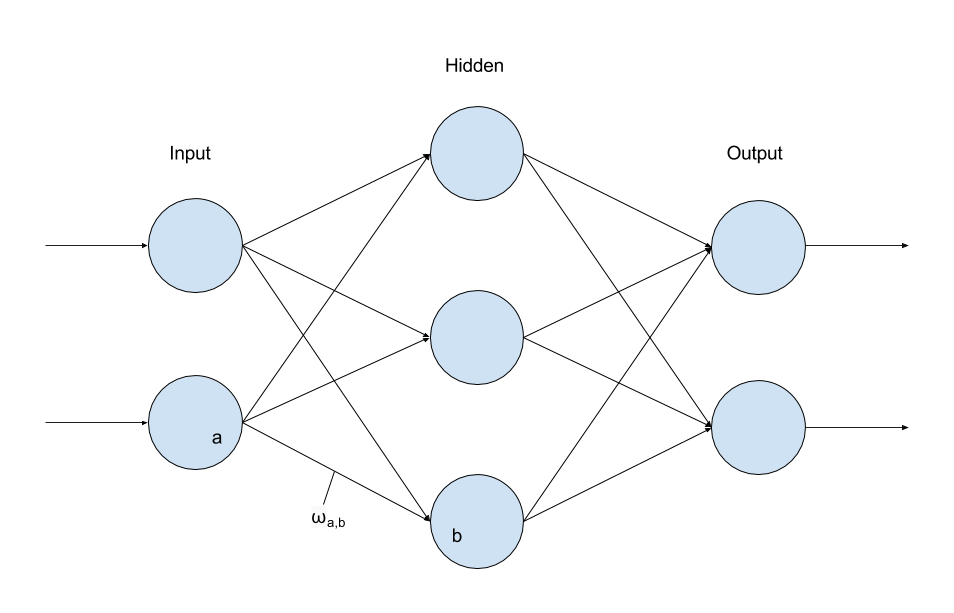
\includegraphics[width=10cm]{fig/MLP_demo}
\caption{Illustrating the preliminary implementation of a three-layer ANN.}
\label{fig:MLP_demo}
\end{figure}

During execution, what happens is that every data point is fed forward through the input layer of the ANN and propagated to the output layer. Following, the squared error of the Euclidean distance between the prediction and the actual data point is calculated. This is used as the erro measure, frmo which a gradient is calculated, used in minimizing the SE. The minimization takes place by updating the weight matrix (one vector per layer of weights) according to the gradient and a learning rate $\alpha$. From this the network extracts a separating hyperplane which minimizes the sum of squares errors for the data set. Note that only a local minimum in the weight space is guaranteed to be found.

\subsection{Results}

During the training phase as outlined above, the FFBP ANN extracted two means which minimizes the error criterion, effectively creating two clusters. Below are the results of the execution process, as well as the results for the toy-example.


\begin{table}
\begin{center}
    \begin{tabular}{ | l | l | l | l |}
    \hline
    \textbf{Measure (seconds)} & \textbf{GPU} & \textbf{CPU} \\ \hline
     Setup, $N=10 000$ & $\approx0.8$ & $\approx7.0$ \\ \hline
     Training, 1k iterations &  $\approx1.5$ & $\approx9.0$ \\ \hline
     Training, 10k iterations &  $\approx14.6$ & $\approx65.8$ \\ \hline
    \end{tabular}
\end{center}
\caption{Presenting the results from running the MLP as elaborated on above on two data-sets consisting of $N=10 000$ two-dimensional data points, training for $1000$ and $10 000$ iterations. Note that the execution time was about 4-6 times faster when running on a GPU, and this is for a non-optimized version of the algorithm. See figure \ref{fig:theano_mlp_demo} for a plot of the results.}
\label{tab:MLP_gpu_vs_cpu}
\end{table}

Note that the results of table \ref{tab:MLP_gpu_vs_cpu} only presents a performance increase of slightly less than an order of magnitude for using the GPU. It is important to emphasise that we cannot given the architecture of an ANN model achieve a performance increase which is greater than the relative number of neurons in the network, which are the highly decentralizable units (i.e the size of the matrices that we operate on). Thus the performance increase as seen in table \ref{tab:MLP_gpu_vs_cpu} for the preliminary implementation suggests that it is fairly optimal in terms of parallelization, given the network size and performance gain when using the GPU.

\begin{figure}
\centering
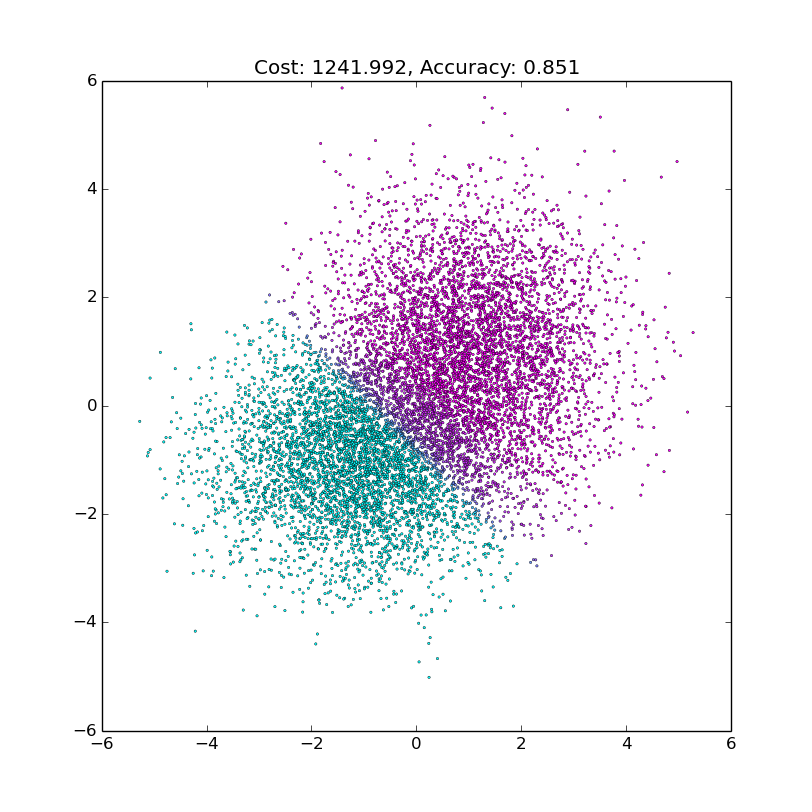
\includegraphics[width=12cm]{fig/MLP_cluster_N_10000_1kiter}
\caption{Illustrating the final plot after training for $10 000$ iterations on a data set with $N=10 000$ normally distributed two-dimensional data points. The cost is the sum of squared errors of the Euclidean distance between the predicted data points and the actual data points, and the accuracy is the relative frequency of correctly classified data points. Note the blue line between the two clusters, which results from data points being classified into the two different classes on top of each other, resulting into blue when the colours blend. This line is in fact representing the separating hyperplane (linear separator in this case).}
\label{fig:theano_mlp_demo}
\end{figure}

In this implementation, BP is performed layer-wise, actually taking into account the current gradient when using the chain-rule for back-propagation of the error signal throughout the network. 
However, it is possible to show that convergence can be guaranteed for certain conditions even when using former time-steps in back-propagating gradients ([ref]). Note that because of these algorithmic implications, the algorithm would also be tolerant towards the potential aliasing of weights in shared memory! However, this should of course be avoided if possible.
However, it actually suggests that the algorithm could be optimized in terms of using former error-gradients when calculating the updates. Note however, that this increases the number of iterations required for convergence and a satisfactory accuracy, particularly in the case of attempting to segment randomly distributed data. This may be seen by considering that the nature of a data set will affect the gradient calculation and convergence.

\cleardoublepage